\documentclass[11pt,a4paper]{article}
\usepackage[margin=14mm,top=12mm,bottom=14mm]{geometry}
\usepackage{graphicx,xcolor,tabularx,booktabs,array,enumitem,ragged2e}
\usepackage[T1]{fontenc}
\usepackage{lmodern}
\usepackage{microtype}
\usepackage{fancyhdr}
\usepackage[hidelinks]{hyperref}
\setlength{\parindent}{0pt}
\setlength{\parskip}{4pt}
\setlist[itemize,enumerate]{leftmargin=5mm,itemsep=1.5pt,topsep=2pt}
\definecolor{navy}{HTML}{17365D}
\definecolor{blue}{HTML}{2F75B5}
\definecolor{green}{HTML}{548235}
\definecolor{amber}{HTML}{BF8F00}
\definecolor{red}{HTML}{C00000}
\definecolor{gray}{HTML}{666666}
\definecolor{palegreen}{HTML}{EAF2E3}
\definecolor{paleblue}{HTML}{E7F0F8}
\definecolor{paleamber}{HTML}{FFF3D6}
\definecolor{palered}{HTML}{FBE5E5}
\definecolor{palegray}{HTML}{EEEEEE}
\newcommand{\boxx}[2]{\noindent\colorbox{#1}{\parbox{\dimexpr\linewidth-2\fboxsep}{#2}}}
\newcommand{\tagg}[2]{\colorbox{#1}{\strut\textcolor{white}{\bfseries\scriptsize #2}}}
\newcommand{\heading}[1]{{\color{navy}\LARGE\bfseries #1}\par\vspace{2mm}\color{blue}\rule{\linewidth}{1.2pt}\color{black}\vspace{2mm}}
\newcommand{\metric}[2]{\begin{minipage}[t]{0.19\linewidth}\centering{\color{navy}\Large\bfseries #1}\\[-1mm]\footnotesize #2\end{minipage}}
\pagestyle{fancy}\fancyhf{}
\lhead{\footnotesize Supervisor progress update}\rhead{\footnotesize 24 July 2026}
\cfoot{\footnotesize\thepage\ / 7}
\renewcommand{\headrulewidth}{0.3pt}
\begin{document}

\thispagestyle{fancy}
{\color{navy}\huge\bfseries Progress Report:\par}
{\color{navy}\LARGE\bfseries Adaptive Remeshing, Mesh Refinement, and State Transfer\par for Phase-Field Fracture Simulations in Abaqus\par}
\vspace{3mm}
{\large Master Thesis Technical Progress and Current Evidence Boundary}

\begin{tabularx}{\linewidth}{@{}lX@{}}
\textbf{Author} & Pruthviraja Reddy Vandavagali\\
\textbf{Programme} & Master Thesis, TU Bergakademie Freiberg\\
\textbf{Report date} & 24 July 2026\\
\textbf{Frozen evidence revision} & \texttt{c34a944da4d01ba6a694878104b0c10c3d87f24e}\\
\end{tabularx}

\heading{Executive summary}
The objective is to establish when localized mesh refinement and state transfer can be used reliably in phase-field fracture simulations, and to document explicit stopping criteria where the evidence is insufficient. This matters because refinement alone is not useful unless history, irreversibility, solver ingestion, and continuation remain controlled.

\boxx{palegreen}{\textbf{\color{green}Main achievement}\quad A reproducible MISESERI pre-refinement and bounded state-transfer workflow was developed and tested.}
\boxx{paleblue}{\textbf{\color{blue}Strongest validated scope}\quad Elastic, pre-peak, and peak response; controlled state ingestion; bounded pre-peak nonmatching transfer.}
\boxx{palered}{\textbf{\color{red}Main current limitation}\quad The corrected D3D-A1 candidate is mathematically admissible under frozen history but is not a mechanically validated Abaqus restart.}

\small
\begin{tabularx}{\linewidth}{@{}X>{\raggedleft\arraybackslash}p{43mm}@{}}
\toprule
\textbf{Project area} & \textbf{Current status}\\ \midrule
Environment and published framework & \tagg{green}{COMPLETED}\\
Offline MISESERI refinement & \tagg{green}{COMPLETED IN SCOPE}\\
Bounded state transfer & \tagg{green}{VALIDATED PRE-PEAK}\\
Active-set correction & \tagg{green}{VALIDATED OFFLINE}\\
Corrected mechanical restart & \tagg{gray}{UNPROVEN}\\
Online adaptive remeshing & \tagg{gray}{NOT VALIDATED}\\
Thesis writing and supervisor review & \tagg{blue}{ONGOING}\\ \bottomrule
\end{tabularx}
\normalsize
\boxx{paleamber}{\textit{The contribution is not merely a refined crack simulation. It is an evidence-driven workflow showing where refinement and transfer are reliable, where they fail, and how the workflow can be controlled reproducibly.}}

\clearpage
\heading{Overall workflow and completed stages}
\begin{center}
\includegraphics[width=\linewidth,height=0.70\textheight,keepaspectratio]{../../results/supervisor_progress_update/figures/combined_project_workflow.pdf}
\end{center}
\boxx{paleblue}{\textbf{Reading the workflow.} Green denotes evidence validated within its tested scope; amber marks conditional support or a disproven continuation assumption; gray/red marks a withheld result or qualification limitation. Internal stage identifiers are retained only in the evidence package.}
\vfill
\footnotesize The workflow progresses from technical reproduction through MISESERI-based offline refinement to transfer and active-set qualification. No online adaptive-remeshing claim is made.

\clearpage
\heading{Stage C -- MISESERI offline refinement}
\begin{center}
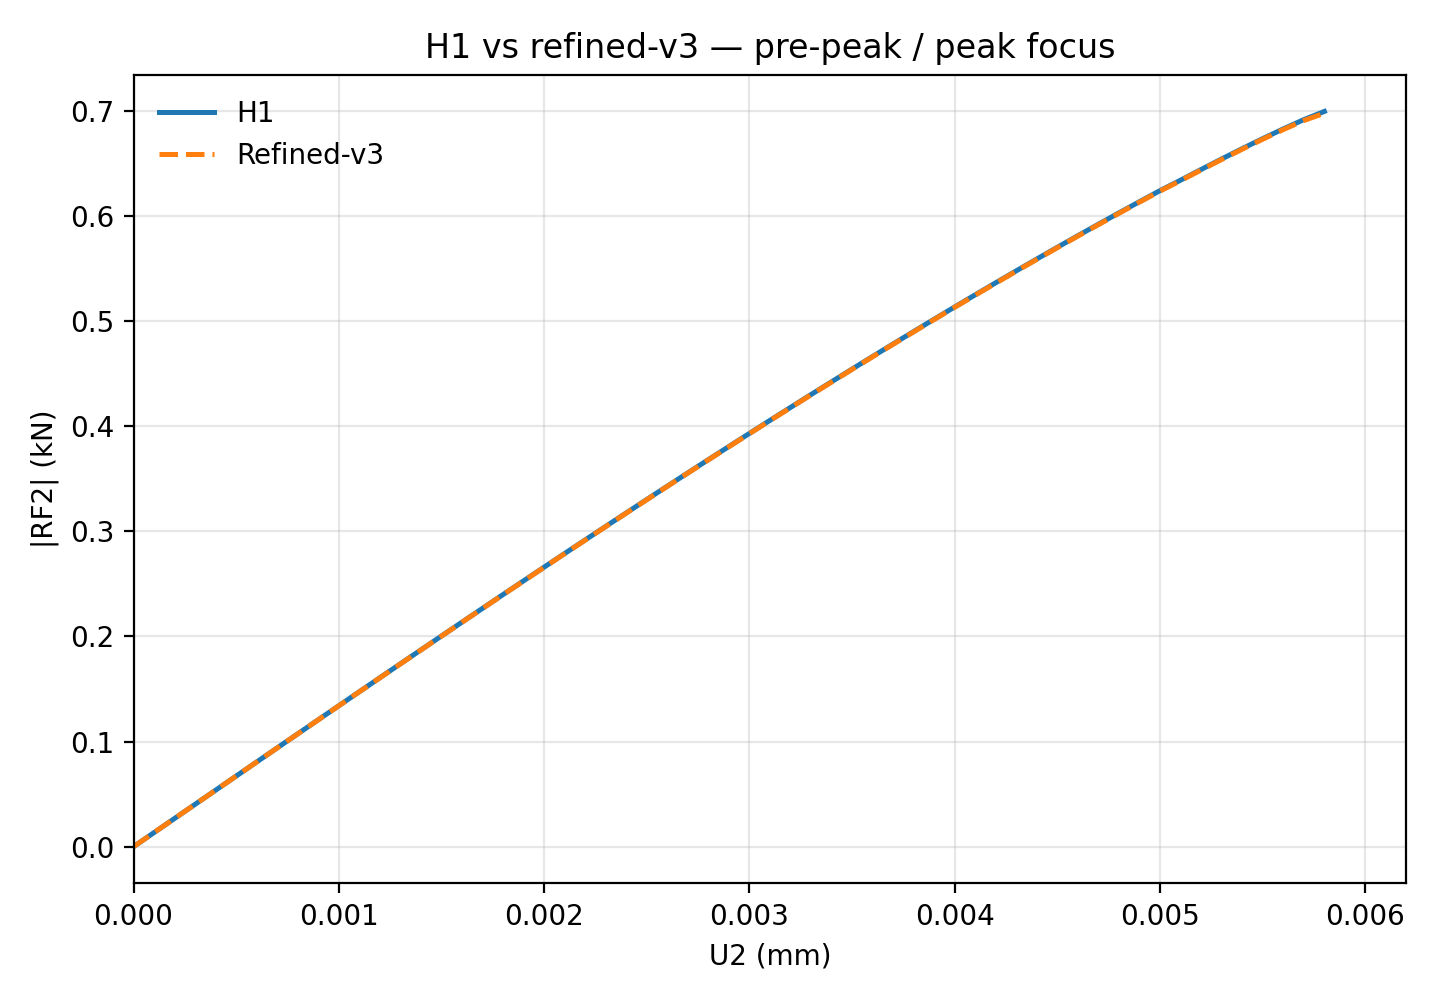
\includegraphics[width=.55\linewidth]{../../results/figures/stage_c_final/02_rf_u_h1_vs_refined_v3_prepeak.png}\hfill
\includegraphics[width=.42\linewidth]{../../results/supervisor_progress_update/figures/stage_c_efficiency_reductions.pdf}
\end{center}
\vspace{1mm}
\metric{0.061\%}{initial stiffness difference}\hfill
\metric{0.089\%}{pre-peak NRMSE}\hfill
\metric{0.24\%}{peak-force difference}\hfill
\metric{unchanged}{peak displacement}\hfill
\metric{10,290}{elements vs.\ 12,064}

\vspace{4mm}
\boxx{palered}{\textbf{\color{red}Limitation -- post-peak equivalence is not established.} Post-peak normalized root-mean-square error (NRMSE) is approximately 24.3\%, and a crack-path deviation from H1 was detected.}
\vspace{2mm}
\boxx{palegreen}{\textbf{Conclusion.} Supported for elastic, pre-peak, and peak response within the tested parameter set; not supported as a crack-path-equivalent replacement for H1.}
\vfill
\footnotesize RF--U denotes reaction force versus displacement. Cost reductions compare refined-v3 with the four-thread H1 reference: physical elements 14.7\%, wall time 16.7\%, CPU time 14.9\%, and peak memory 22.2\%.

\clearpage
\heading{Stage D -- state transfer\\and Abaqus ingestion}
\boxx{paleblue}{\centering\bfseries Controlled analytical transfer $\rightarrow$ Abaqus ingestion $\rightarrow$ Serial continuation\\[1mm]
$\rightarrow$ Four-thread repeatability $\rightarrow$ Nonmatching checkpoint transfer $\rightarrow$ Compatible release hold}

\vspace{4mm}
\begin{tabularx}{\linewidth}{@{}Xr@{}}
\toprule
\textbf{Measured quantity} & \textbf{Value}\\ \midrule
Controlled phase $L_2$ error & 0.027037\\
Controlled phase maximum error & 0.084997\\
Controlled history $L_2$ error & 0.010797\\
Controlled history maximum error & 0.023398\\
Target checkpoint nodes & 6,601\\
Physical elements / integration points & 6,400 / 25,600\\
R4 SDV15 maximum transfer error & $1.3878\times10^{-17}$\\
R4 SDV16 maximum transfer error & 0\\
Relative reaction-force release jump & $2.2926\times10^{-4}$\\
Relative energy release jump & $1.2746\times10^{-5}$\\ \bottomrule
\end{tabularx}

\vspace{4mm}
\boxx{paleamber}{\textbf{Interpretation.} The analytical transfer errors are measured and retained as a baseline; they are not described as negligible. Abaqus ingestion, serial/four-thread continuation, bounded nonmatching pre-peak transfer, and the compatible R4 release hold passed their declared gates.}
\vfill
\footnotesize SDV denotes a solution-dependent variable. The user element (UEL), user material (UMAT), and MISESERI pre-analysis form the controlled implementation chain.

\clearpage
\heading{Active-set evolution and offline correction}
\begin{center}
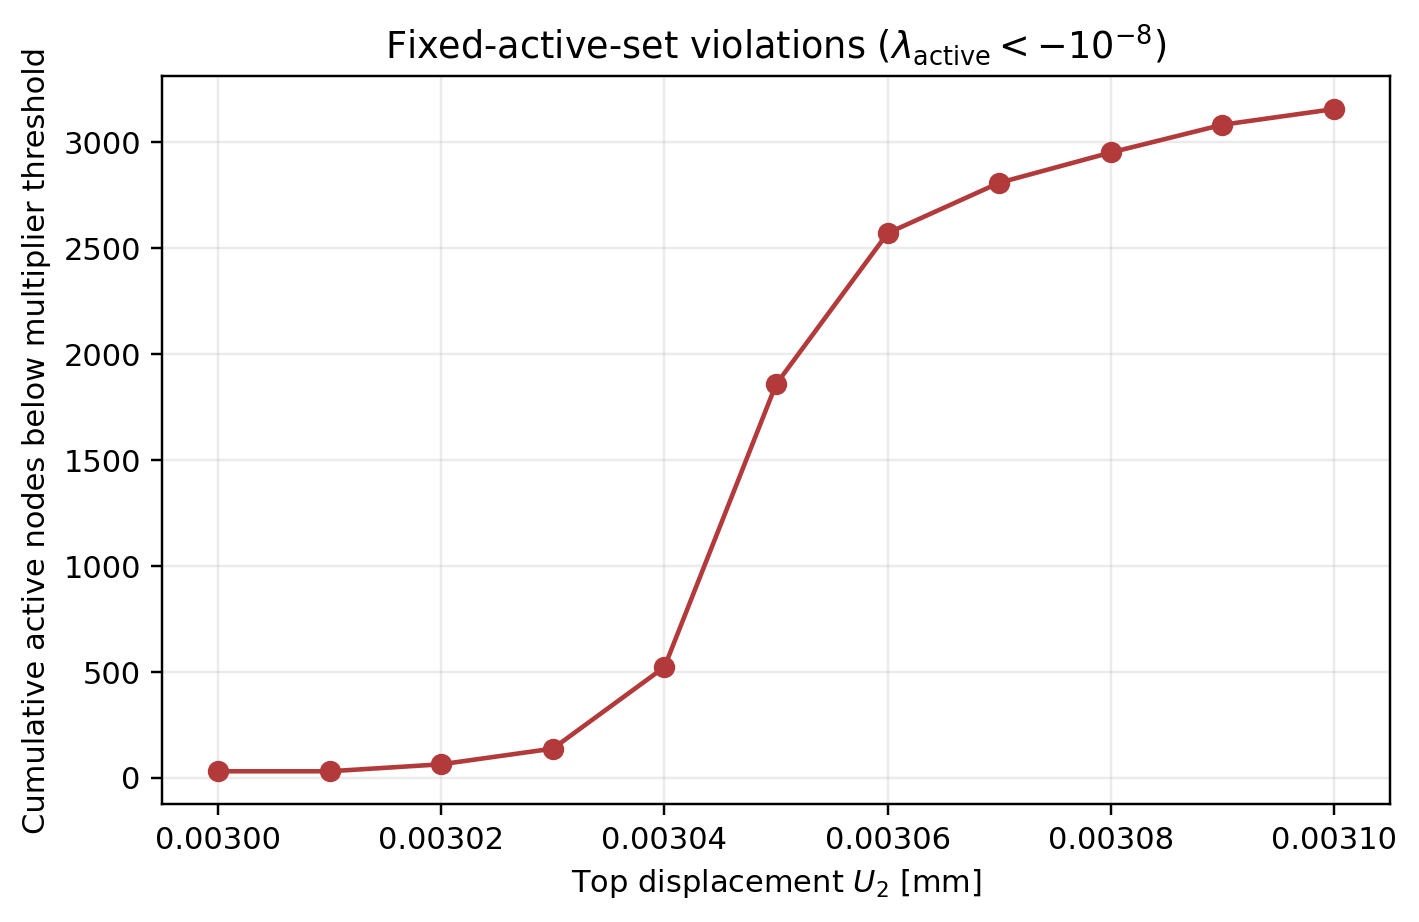
\includegraphics[width=.72\linewidth,height=.27\textheight,keepaspectratio]{../../results/final/stage_d/figures/violating_active_nodes_vs_displacement.png}\\[-1mm]
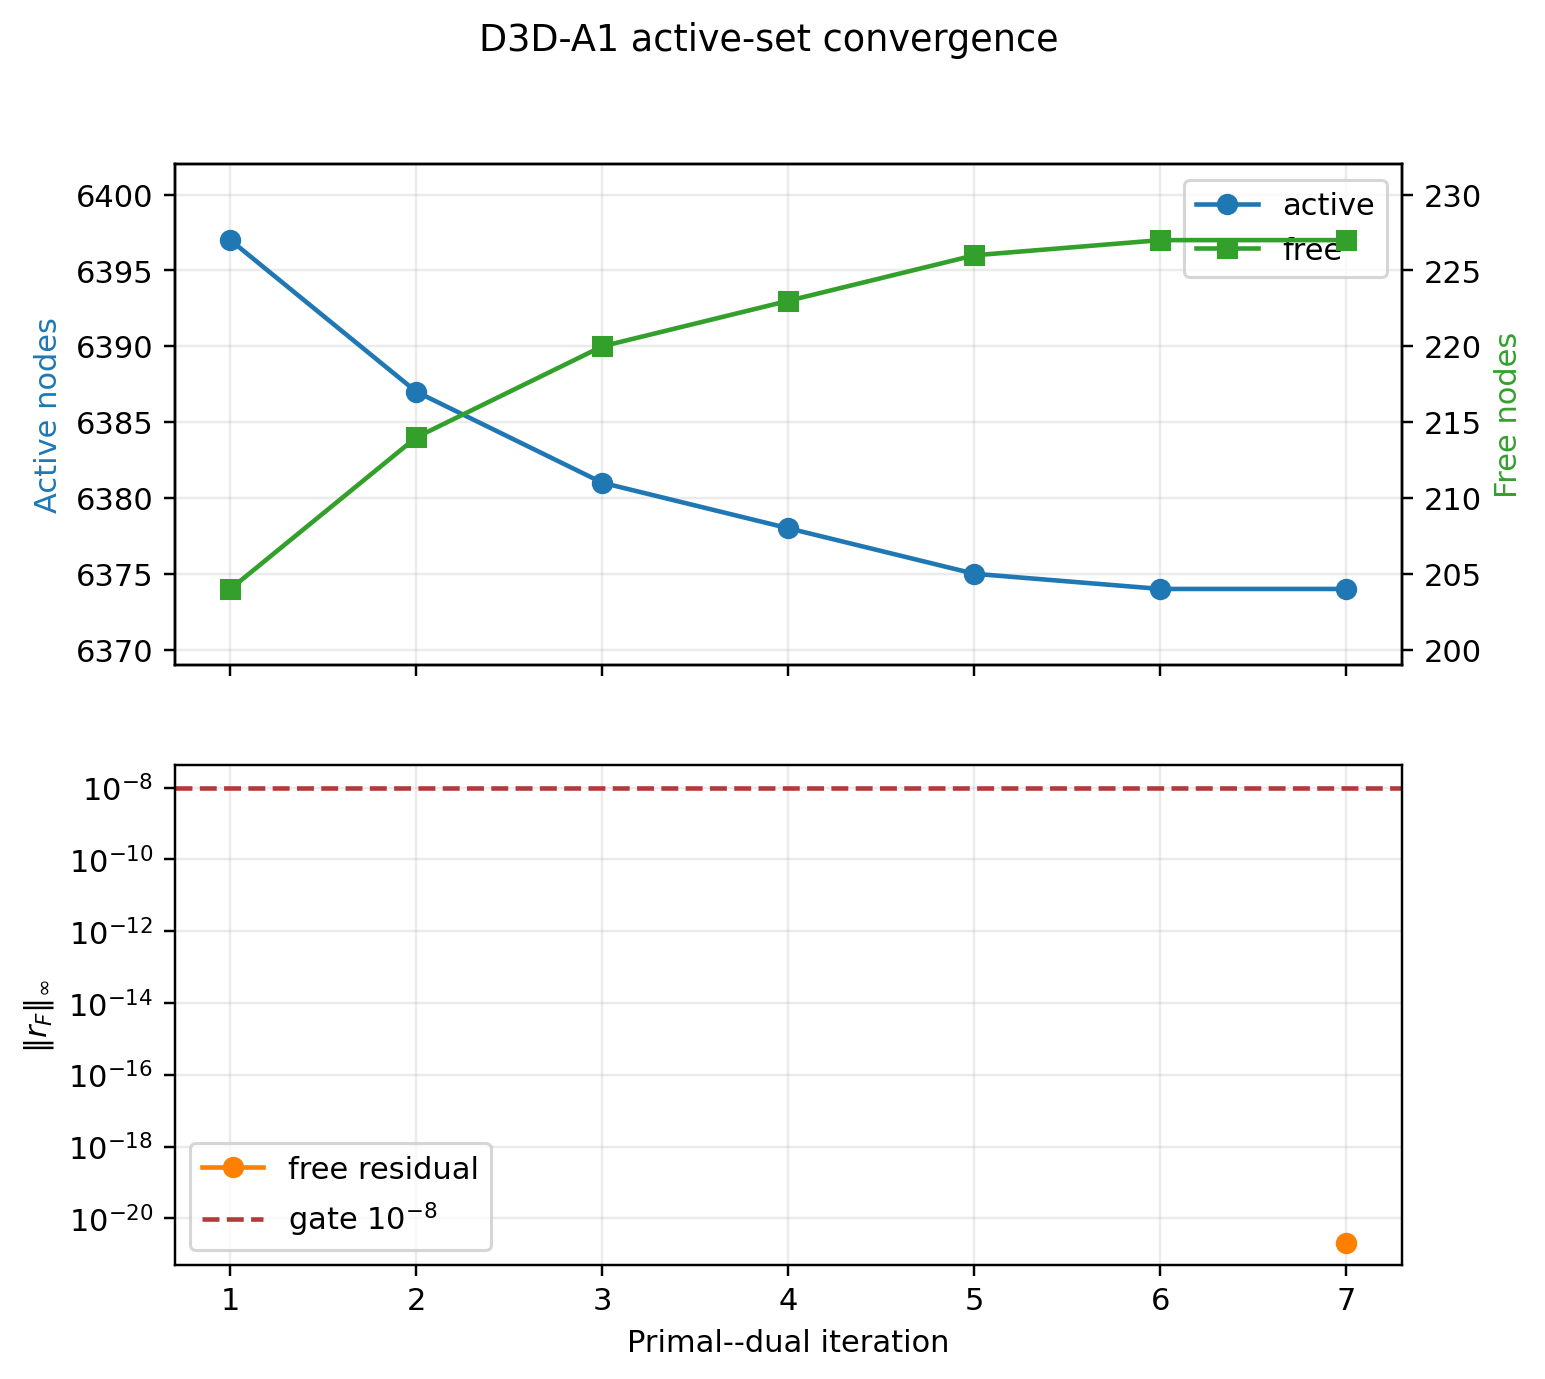
\includegraphics[width=.62\linewidth,height=.23\textheight,keepaspectratio]{../../results/final/stage_d/figures/d3d_a1_active_set_convergence.png}
\end{center}
\begin{minipage}[t]{.48\linewidth}
\boxx{paleamber}{\textbf{Fixed active-set test}\\
30 violating active nodes initially\\
3,157 violating nodes at endpoint\\
Minimum multiplier: $-1.8327\times10^{-7}$\\[1mm]
\textbf{Disproven:} one fixed active set cannot be carried through the tested loading segment.}
\end{minipage}\hfill
\begin{minipage}[t]{.48\linewidth}
\boxx{palegreen}{\textbf{Offline correction}\\
7 deterministic iterations; 6,374 active / 227 free\\
72 releases: 30 seeds + 42 additional; no reactivation\\
Free residual: $2.1176\times10^{-21}$\\
Minimum multiplier: $-9.99696\times10^{-9}$\\
Zero bound error; no phase decrease or non-positive Jacobian.}
\end{minipage}
\vspace{3mm}
\boxx{palegreen}{\textbf{The corrected phase field is KKT-admissible under the frozen F3 history.}}
\boxx{palered}{\textbf{This does not prove that the corrected package is an accepted mechanical restart.}}
\vfill
\footnotesize KKT denotes Karush--Kuhn--Tucker optimality conditions. The active-multiplier acceptance threshold is $-10^{-8}$.

\clearpage
\heading{Qualification failures and scientific interpretation}
\begin{center}
\includegraphics[width=\linewidth]{../../results/supervisor_progress_update/figures/qualification_failure_timeline.pdf}
\end{center}
\boxx{palegray}{All three jobs stopped before Abaqus because of wrapper or environment failures. None produced a solver or scientific result. They do not contradict the successful offline correction; mechanical re-equilibration remains unknown.}

\begin{minipage}[t]{.48\linewidth}
\boxx{palegreen}{\textbf{\color{green}What is proven}\\
\begin{itemize}
\item published framework technically reproducible;
\item Stage C peak/pre-peak response;
\item controlled state ingestion;
\item bounded nonmatching pre-peak transfer;
\item R4 release hold;
\item offline correction under frozen history.
\end{itemize}}
\end{minipage}\hfill
\begin{minipage}[t]{.48\linewidth}
\boxx{palered}{\textbf{\color{red}Not proven or withheld}\\
\begin{itemize}
\item corrected mechanical restart;
\item D3E;
\item post-peak equivalence;
\item online adaptive remeshing;
\item ABAQUSER comparison.
\end{itemize}}
\end{minipage}
\vfill
\footnotesize Qualification records: jobs 1378003--1378005. Retry authorization is exhausted; no further computation is authorized by this report.

\clearpage
\heading{Decisions taken and proposed next work}
\begin{minipage}[t]{.48\linewidth}
\boxx{paleblue}{\textbf{\color{blue}Track A -- Technical qualification}\\
\begin{enumerate}
\item Build a trivial one-element environment package.
\item Pre-stage every required file on the login node.
\item Use no Git command on the compute node.
\item Bind Python, compiler, and Abaqus explicitly.
\item Run only a trivial user-subroutine datacheck.
\item Preserve complete success/failure evidence.
\item Reconsider checkpoint qualification only after this independent gate passes.
\end{enumerate}}
\end{minipage}\hfill
\begin{minipage}[t]{.48\linewidth}
\boxx{palegreen}{\textbf{\color{green}Track B -- Thesis development}\\
\begin{enumerate}
\item Obtain comments on the consolidated tolerance policy.
\item Integrate validated results into the university thesis template.
\item Finalize literature, discussion, conclusions, and outlook.
\item Prepare the defense presentation.
\item Keep every unsupported claim explicitly withheld.
\end{enumerate}}
\end{minipage}

\vspace{6mm}
\boxx{paleamber}{\Large\bfseries The current work establishes a reproducible and bounded workflow for MISESERI-based offline refinement and pre-peak state transfer, while exposing the active-set and infrastructure limitations that must be resolved before validated online continuation.}

\vfill
\small\textbf{Evidence boundary.} This brief summarizes committed evidence frozen at revision\\
\texttt{c34a944da4d01ba6a694878104b0c10c3d87f24e}. It is a progress report, not the final thesis. Detailed metrics, provenance, tolerance decisions, and withheld claims remain in the frozen evidence package.

\end{document}
